% !TEX program = xelatex
\documentclass{misisarticle}

\grnti{28.23.15, 27.47.19}
\asjc{1707, 1702}
\oecd{1.02}

\makeatletter
\renewcommand{\@authorcolumns}{%
  \begin{center}
    \misis@authorsleft
  \end{center}%
}
\makeatother

\title{Классификация 3D-моделей объектов культурного наследия по облакам точек на основе нейросетевых подходов}

\misisauthor{С.~М.~Хлобустова}{кафедра инженерной кибернетики НИТУ «МИСиС»}{Москва, Россия}{m2104526@edu.misis.ru}

\setabstract{В работе проводится сравнительное исследование трёх архитектур обработки облаков точек — PointNet, DGCNN и SA-MLP — в задаче классификации 3D-моделей объектов культурного наследия. Модели обучены на подмножестве ModelNet40 (пять классов сосудов-артефактов) и оценены в трёх режимах: на чистых синтетических данных, при контролируемом гауссовом шуме и на независимом наборе из 50 реальных 3D-сканов музейных предметов. Установлено, что при близкой точности на чистых данных (84.6--86.9\%) архитектуры кардинально различаются по устойчивости: DGCNN сохраняет точность при переносе на реальные сканы (−0.9 п.п.), тогда как PointNet и SA-MLP теряют около 30 п.п., что противоположно их поведению при синтетическом зашумлении. Таким образом, DGCNN демонстрирует наилучшую практическую применимость для классификации реальных 3D-сканов объектов культурного наследия.}
\setkeywords{DGCNN, ModelNet40, PointNet, доменный сдвиг, классификация 3D-объектов, компьютерное зрение, облака точек, set-abstraction, устойчивость к шуму}

\begin{document}
\maketitle

\section{Введение}

Обработка трёхмерных данных методами глубокого обучения приобретает всё большее значение в задачах распознавания объектов, робототехники, автономного транспорта и цифровизации культурного наследия. В отличие от двумерных изображений, представленных регулярной сеткой пикселей, трёхмерные объекты допускают несколько форм представления: воксельные сетки, полигональные меши, облака точек и множественные 2D-проекции [1]. Облако точек — набор точек, заданных координатами $(x,y,z)$ на поверхности объекта, — является форматом, близким к сырым данным сканеров и лидаров, и не требует предварительной вокселизации.

Ключевая трудность обработки облаков точек состоит в их неупорядоченности: облако инвариантно к перестановке точек, поэтому классические свёрточные сети неприменимы к нему напрямую. Одной из первых архитектур, работавших непосредственно с сырыми точками, стала PointNet [2]. Последующие работы — PointNet++ [3], DGCNN [4], Point Transformer [5] — развивали идею учёта локальной геометрии, что существенно расширило возможности обработки точечных данных.

Большинство исследований оценивают архитектуры на синтетических наборах ModelNet40 [6] и ShapeNet [7], состоящих из CAD-моделей. Реальные сканы музейных экспонатов содержат неравномерную плотность точек, шум, пропуски и артефакты реконструкции. Вопрос о том, насколько точность на синтетических данных предсказывает поведение модели в реальных условиях, определяет практическую применимость методов в задачах цифровизации культурного наследия [8]. Обработка облаков точек от реальных сенсоров требует учёта их специфики — неравномерной плотности, шума и пропусков [16,18]. Методология сравнительной оценки нескольких архитектур по единому протоколу применялась и в работах студентов кафедры: в [19] проведено сравнение двух версий детектора YOLO по точности и скорости в реальном времени, а в [20] решена задача классификации объектов нескольких типов средствами компьютерного зрения с использованием собственного набора данных.

Настоящая работа ставит следующие исследовательские вопросы:
\begin{enumerate}
  \item Как выбор архитектурного подхода влияет на точность классификации 3D-моделей артефактов при прочих равных условиях?
  \item Какая архитектура наиболее устойчива к синтетическому гауссову шуму во входных координатах точек?
  \item Сохраняется ли ранжирование архитектур при переходе от синтетических данных к реальным фотограмметрическим сканам?
\end{enumerate}

Для ответа на эти вопросы обучены три архитектуры, проведены эксперименты с контролируемым шумом и подготовлен независимый набор реальных сканов.

\section{Наборы данных}

\subsection{Обучающий набор — ModelNet40}

Для обучения использовалось подмножество ModelNet40 [6], содержащего 12\,311 CAD-моделей 40 категорий. Применялась предобработанная версия с облаками из 2048 точек [4]. Отобраны пять классов сосудов-артефактов: \textit{bottle}, \textit{bowl}, \textit{cup}, \textit{flower\_pot}, \textit{vase}. Использовался стандартный официальный split.

\begin{table}[htbp]
\caption{Структура обучающего подмножества ModelNet40}
\label{tab:modelnet}
\centering
\begin{tabular}{lcc}
\toprule
Класс & Обучающая & Тестовая \\
\midrule
\textit{bottle} & 335 & 100 \\
\textit{bowl} & 64 & 20 \\
\textit{cup} & 79 & 20 \\
\textit{flower\_pot} & 149 & 20 \\
\textit{vase} & 475 & 100 \\
\midrule
Всего & 1\,102 & 260 \\
\bottomrule
\end{tabular}
\end{table}

Выборка несбалансирована: классы \textit{vase} и \textit{bottle} доминируют. Классы близки по форме и различаются локальными деталями, например ручкой у \textit{cup} и формой горла у \textit{vase} и \textit{flower\_pot}, что делает задачу нетривиальной.

\begin{figure}[htbp]
  \centering
  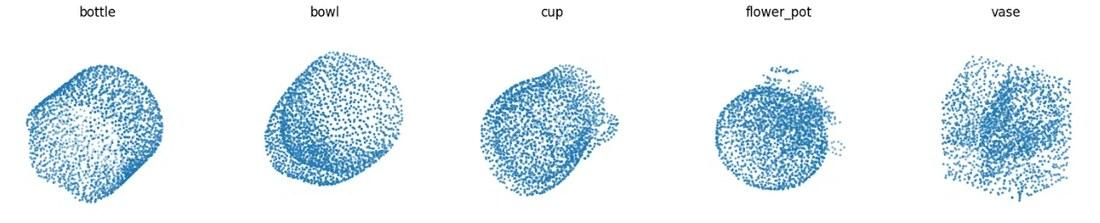
\includegraphics[width=\columnwidth]{figures/fig01.jpg}
  \caption{Примеры облаков точек пяти классов из ModelNet40: \textit{bottle}, \textit{bowl}, \textit{cup}, \textit{flower\_pot}, \textit{vase}}
  \label{fig:modelnet}
\end{figure}

\subsection{Собственный набор реальных сканов}

Для оценки устойчивости к доменному сдвигу подготовлен независимый тестовый набор из 50 3D-моделей музейных предметов (по 10 на каждый из пяти классов). Модели получены из открытого репозитория Sketchfab, раздел Cultural Heritage, с условиями лицензирования, допускающими использование соответствующих моделей. В отличие от CAD-моделей ModelNet40, эти объекты являются результатом реконструкции реальных предметов и содержат неравномерную плотность точек, шум поверхности, пропуски и артефакты реконструкции.

Каждая модель отнесена к одному из пяти классов вручную. Исходный меш нормирован в единичный куб и сэмплирован в облако из 1024 точек. Набор использовался исключительно на этапе инференса, без дообучения моделей. Датасет размещён публично [22].

\begin{figure}[htbp]
  \centering
  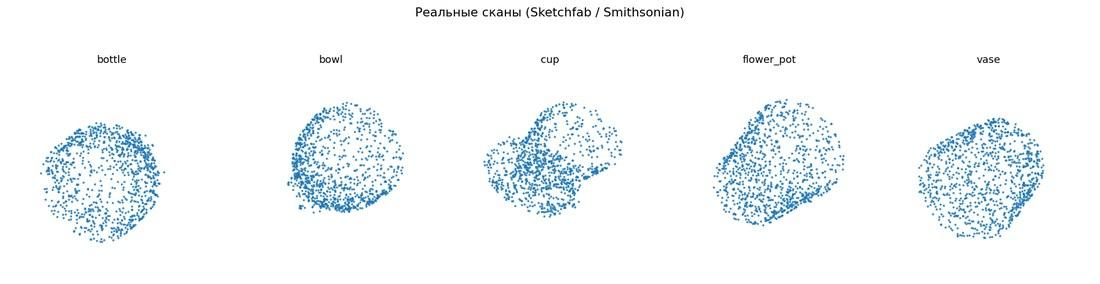
\includegraphics[width=\columnwidth]{figures/fig02.jpg}
  \caption{Примеры облаков точек из собственного набора реальных сканов}
  \label{fig:realdata}
\end{figure}

\section{Исследуемые архитектуры}

Для сравнения выбраны три архитектуры, представляющие различные подходы к обработке облаков точек.

\subsection{PointNet}

PointNet [2] обрабатывает каждую точку независимо серией общих многослойных перцептронов (Conv1d с ядром 1) и агрегирует поточечные признаки в глобальный дескриптор с помощью глобального max-pooling. Для обучения пространственного выравнивания используются обучаемые матрицы T-Net. Модель не учитывает взаимное расположение соседних точек — глобальное агрегирование является её ключевой архитектурной особенностью. Реализация содержит 3.47 млн параметров.

\begin{figure}[htbp]
  \centering
  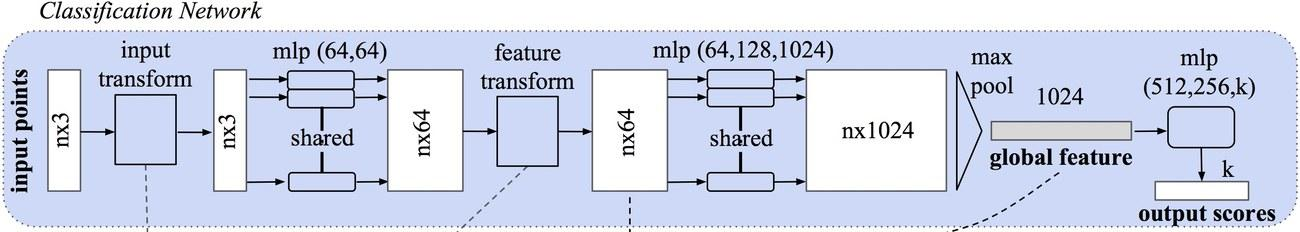
\includegraphics[width=\columnwidth]{figures/fig03.jpg}
  \caption{Архитектура PointNet: поточечные общие MLP, выравнивание T-Net и глобальное max-pooling}
  \label{fig:pointnet}
\end{figure}

\subsection{DGCNN}

DGCNN (Dynamic Graph CNN) [4] строит для каждой точки граф $k$ ближайших соседей и применяет операцию EdgeConv, вычисляющую признаки рёбер как функцию центральной точки и относительного смещения к соседу. Граф перестраивается динамически на каждом слое в пространстве признаков. Финальный дескриптор формируется комбинацией max- и average-pooling. Реализация содержит 1.80 млн параметров при $k=20$.

\begin{figure}[htbp]
  \centering
  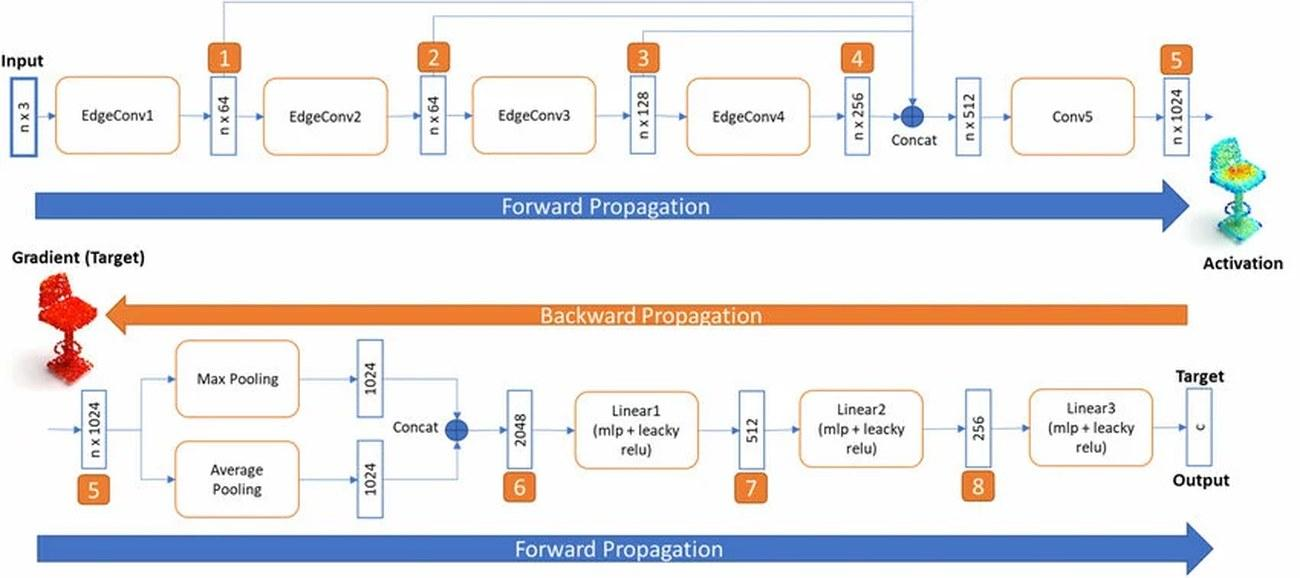
\includegraphics[width=\columnwidth]{figures/fig04.jpg}
  \caption{Архитектура DGCNN: последовательность блоков EdgeConv, конкатенация признаков уровней и агрегация max + average pooling}
  \label{fig:dgcnn}
\end{figure}

\subsection{SA-MLP}

SA-MLP (Set-Abstraction MLP) — иерархическая архитектура на основе механизма set-abstraction [3], в которой последовательно применяются отбор центроидов методом farthest point sampling (FPS), группировка локальных окрестностей процедурой ball query, обработка сгруппированных признаков остаточными MLP-блоками с агрегацией max-pooling. С каждым уровнем число точек уменьшается (1024 $\rightarrow$ 512 $\rightarrow$ 128 $\rightarrow$ 32), а размерность признаков растёт. В отличие от PointNet++, архитектура использует собственную конфигурацию остаточных блоков и параметров группировки. Реализация содержит 1.22 млн параметров — наименьшую из трёх.

\begin{figure}[htbp]
  \centering
  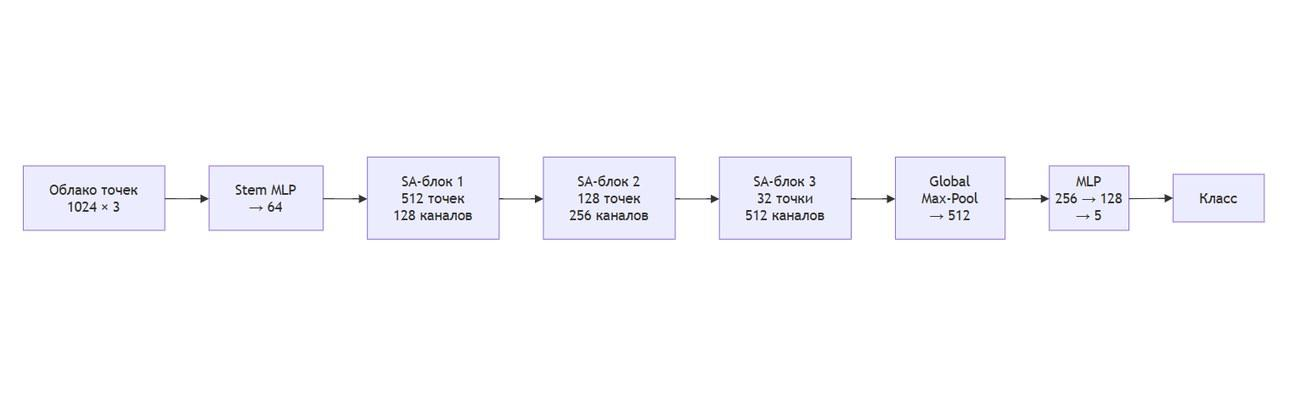
\includegraphics[width=\columnwidth]{figures/fig05.jpg}
  \caption{Архитектура SA-MLP: stem-MLP, три иерархических set-abstraction блока и MLP-классификатор}
  \label{fig:samlp}
\end{figure}

\section{Постановка эксперимента}

\subsection{Обучение}

Все три модели обучены по одному экспериментальному протоколу. Число точек на объект — 1024 (случайное подмножество из 2048). GPU: NVIDIA Tesla T4. Оптимизатор: Adam ($lr_0=1\times10^{-3}$, weight decay $=1\times10^{-4}$). Планировщик: CosineAnnealingLR, 50 эпох. Размер батча: 32. Аугментация: случайный поворот вокруг вертикальной оси и гауссов шум с $\sigma=0.01$. Функция потерь: кросс-энтропия.

\begin{table}[htbp]
\caption{Параметры обучения}
\label{tab:training}
\centering
\begin{tabular}{lc}
\toprule
Параметр & Значение \\
\midrule
Точек на объект & 1\,024 \\
Эпохи & 50 \\
Batch size & 32 \\
Оптимизатор & Adam \\
$lr_0$ / планировщик & $1\times10^{-3}$ / CosineAnnealing \\
Weight decay & $1\times10^{-4}$ \\
Аугментация & поворот + шум ($\sigma=0.01$) \\
GPU & Tesla T4 \\
\bottomrule
\end{tabular}
\end{table}

\subsection{Протокол оценки}

Для устранения неопределённости случайного сэмплинга базовый тестовый набор фиксируется один раз (seed = 42) и используется во всех экспериментах. В эксперименте с шумом к фиксированному тестовому набору добавляется гауссов шум с заданным $\sigma$; результаты усредняются по 10 независимым seed'ам шума и приводятся как mean $\pm$ std. Тест на реальных данных выполняется детерминированно в режиме \texttt{eval()}. Падение точности выражается в процентных пунктах (п.п.).

\subsection{Метрики}

Overall accuracy (OA) используется как основная метрика. Дополнительно рассчитываются per-class F1 и macro-averaged F1 (mF1), то есть среднее значение F1 по классам без учёта их размера. mF1 информативнее OA при дисбалансе классов.

\section{Результаты}

\subsection{Классификация на чистых данных}

Результаты на фиксированной тестовой выборке ModelNet40 приведены в табл.~\ref{tab:clean}. Все три архитектуры показывают близкую точность (84.6--86.9\%), наилучший OA у DGCNN. SA-MLP достигает конкурентного качества при наименьшем числе параметров.

\begin{table}[htbp]
\caption{Сравнение на чистых данных ModelNet40 (test split)}
\label{tab:clean}
\centering
\begin{tabular}{lccc}
\toprule
Модель & Параметры & OA & macro F1 \\
\midrule
PointNet & 3.47 млн & 0.846 & 0.80 \\
DGCNN & 1.80 млн & 0.869 & 0.82 \\
SA-MLP & 1.22 млн & 0.858 & 0.80 \\
\bottomrule
\end{tabular}
\end{table}

\begin{figure}[htbp]
  \centering
  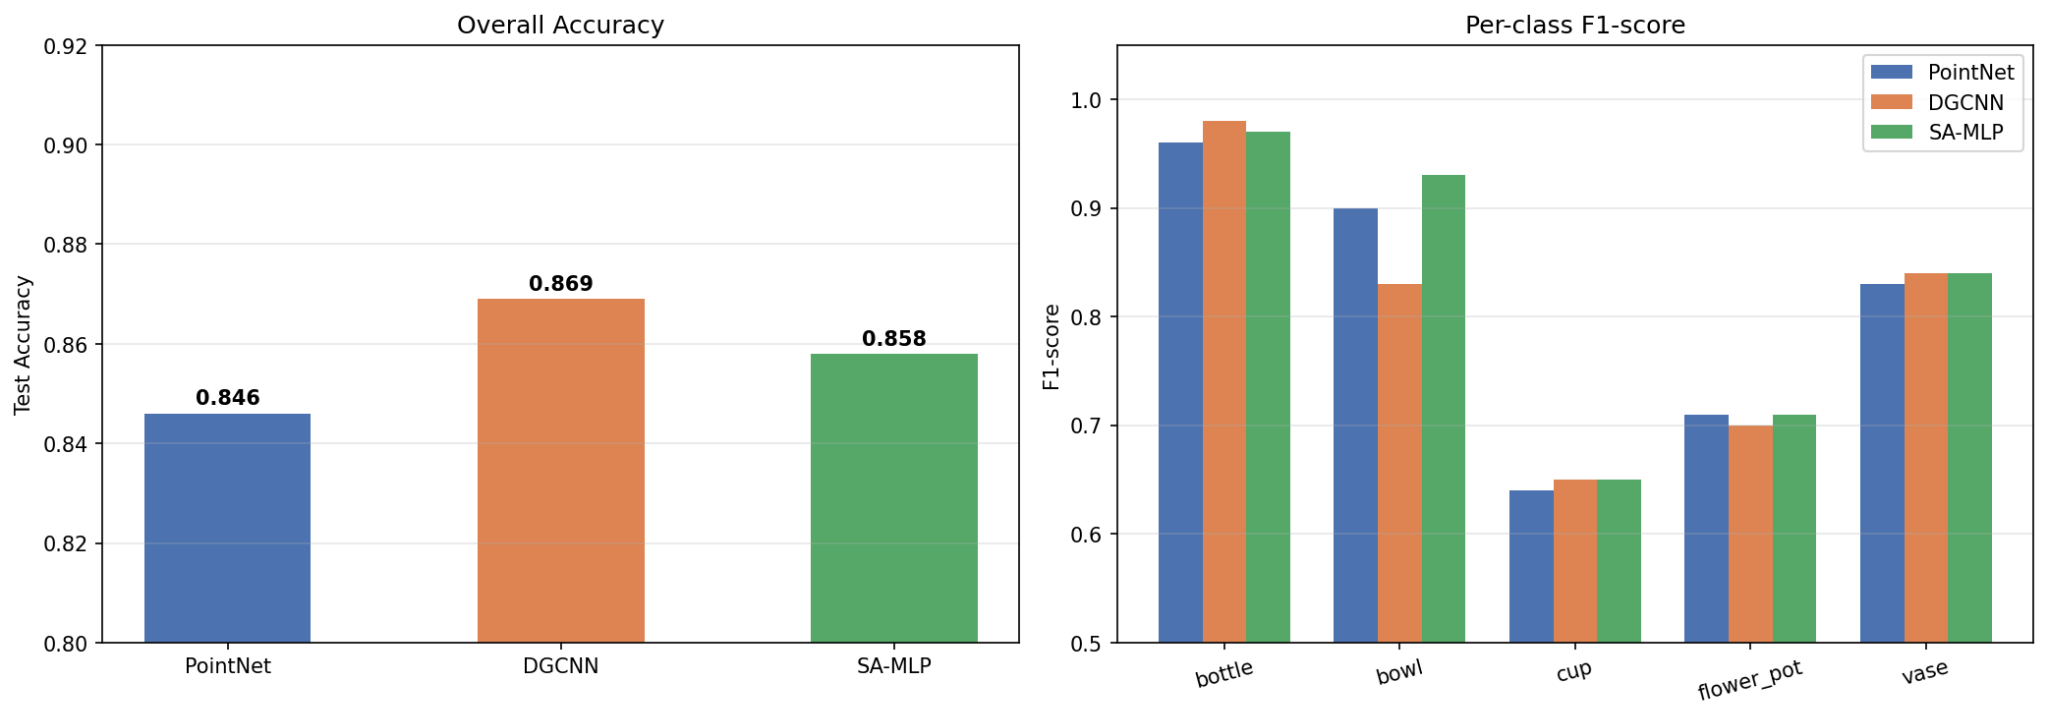
\includegraphics[width=\columnwidth]{figures/fig06.jpg}
  \caption{Overall accuracy и поклассовый F1-score трёх моделей на чистых данных ModelNet40}
  \label{fig:clean}
\end{figure}

Класс \textit{bottle} классифицируется практически идеально всеми моделями (F1 $\geq 0.95$), что может быть связано с его характерным профилем. Класс \textit{cup} — наиболее трудный (F1 = 0.55--0.65): ключевой различающий признак, ручка, занимает малую долю поверхности и может нестабильно попадать в случайную выборку из 1024 точек.

\begin{figure}[htbp]
  \centering
  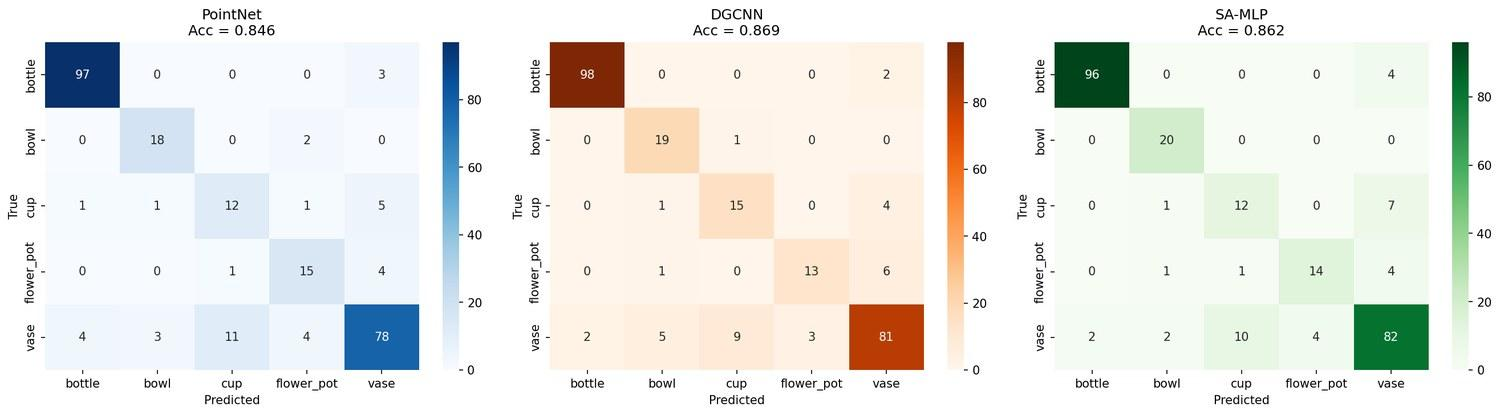
\includegraphics[width=\columnwidth]{figures/fig07.jpg}
  \caption{Матрицы ошибок трёх моделей на чистых данных ModelNet40}
  \label{fig:clean_cm}
\end{figure}

\subsection{Устойчивость к синтетическому шуму}

К фиксированному тестовому набору добавлялся гауссов шум $\sigma$ от 0 до 0.08 в нормированных координатах. Результаты (табл.~\ref{tab:noise}, рис.~\ref{fig:noise}) показывают, что при увеличении уровня шума PointNet деградирует медленнее остальных моделей.

\begin{table}[htbp]
\caption{Accuracy (mean $\pm$ std, 10 seed'ов) при различных $\sigma$}
\label{tab:noise}
\centering
\begin{tabular}{lccc}
\toprule
$\sigma$ & PointNet & DGCNN & SA-MLP \\
\midrule
0.00 & 0.846 & 0.869 & 0.858 \\
0.01 & 0.850 $\pm$ 0.004 & 0.876 $\pm$ 0.006 & 0.863 $\pm$ 0.006 \\
0.02 & 0.854 $\pm$ 0.006 & 0.859 $\pm$ 0.004 & 0.859 $\pm$ 0.007 \\
0.03 & 0.853 $\pm$ 0.009 & 0.823 $\pm$ 0.011 & 0.851 $\pm$ 0.008 \\
0.05 & 0.818 $\pm$ 0.010 & 0.658 $\pm$ 0.016 & 0.795 $\pm$ 0.019 \\
0.08 & 0.686 $\pm$ 0.018 & 0.432 $\pm$ 0.020 & 0.425 $\pm$ 0.011 \\
\bottomrule
\end{tabular}
\end{table}

При $\sigma=0.05$ DGCNN теряет 21.1 п.п., PointNet — лишь 2.8 п.п. При $\sigma=0.08$ DGCNN и SA-MLP деградируют до примерно 43\%, тогда как PointNet сохраняет 68.6\%. Разброс $\pm$std во всех случаях существенно ниже различий между моделями при $\sigma\geq0.05$, что указывает на устойчивость наблюдаемых различий к выбору seed'а шума.

\begin{figure}[htbp]
  \centering
  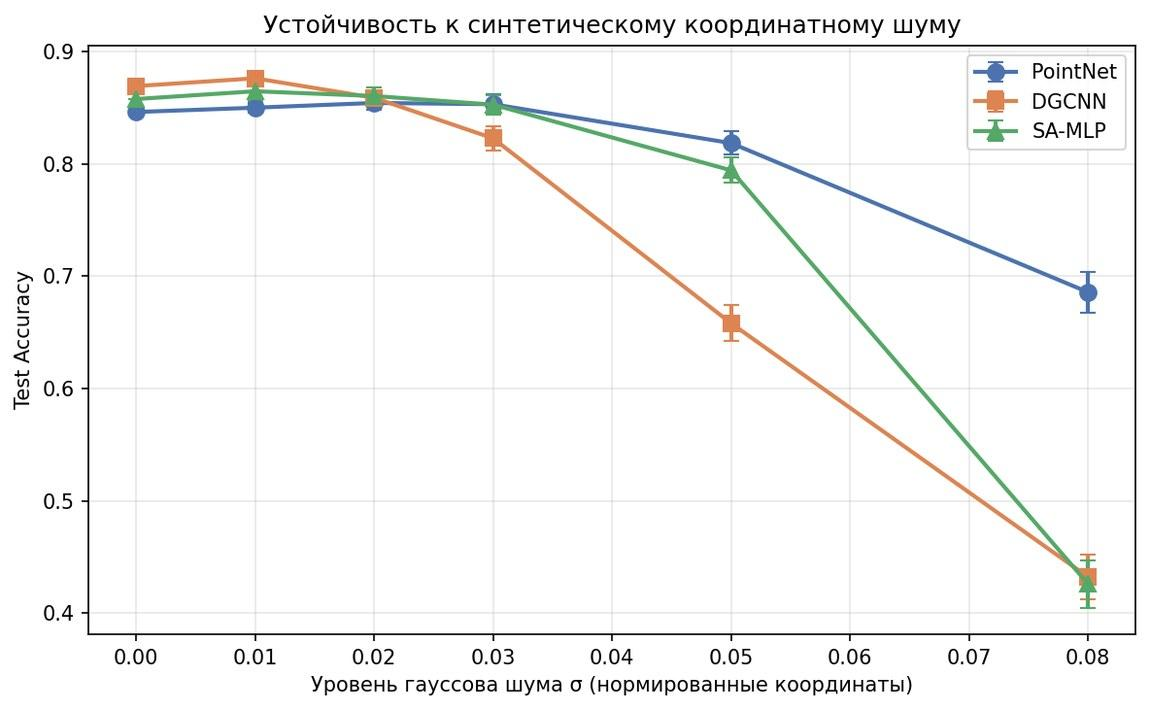
\includegraphics[width=\columnwidth]{figures/fig08.jpg}
  \caption{Устойчивость к синтетическому координатному шуму: accuracy (mean $\pm$ std по 10 seed'ам) в зависимости от $\sigma$}
  \label{fig:noise}
\end{figure}

\subsection{Перенос на реальные сканы}

Оценка на 50 реальных сканах без дообучения даёт картину, противоположную шумовому эксперименту (табл.~\ref{tab:real}, рис.~\ref{fig:domain}).

\begin{table}[htbp]
\caption{Перенос на реальные сканы без дообучения}
\label{tab:real}
\centering
\begin{tabular}{lccc}
\toprule
Модель & Синтетика & Реальные & Падение, п.п. \\
\midrule
PointNet & 0.846 & 0.540 & $-30.6$ \\
DGCNN & 0.869 & 0.860 & $-0.9$ \\
SA-MLP & 0.858 & 0.560 & $-29.8$ \\
\bottomrule
\end{tabular}
\end{table}

DGCNN практически не потерял в точности. PointNet и SA-MLP теряют около 30 п.п., что прямо противоположно результату эксперимента с шумом, где PointNet был наиболее устойчив.

\begin{figure}[htbp]
  \centering
  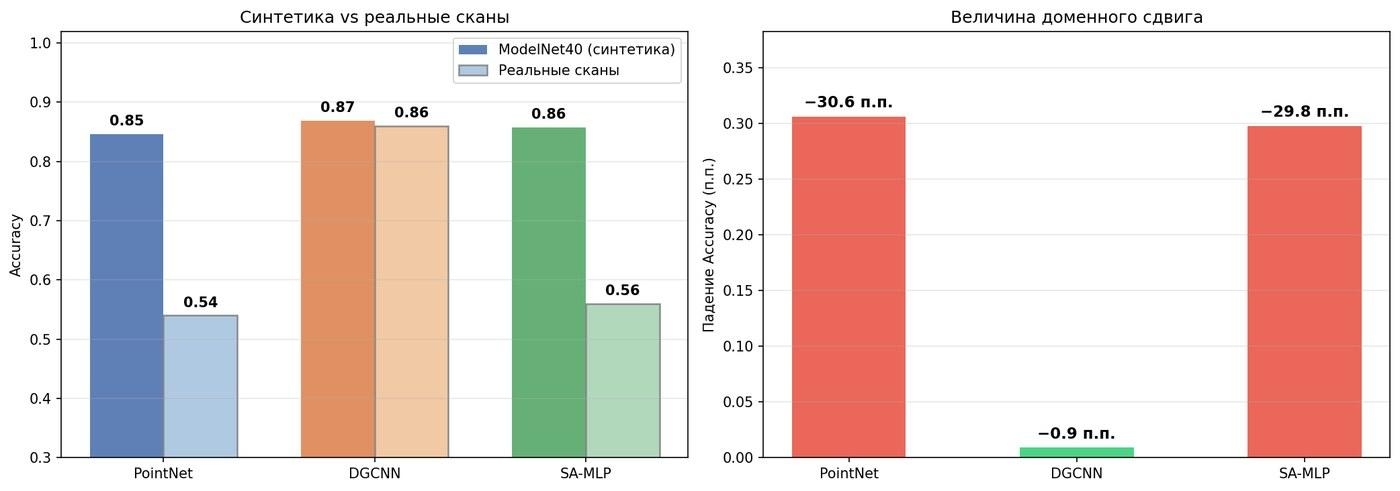
\includegraphics[width=\columnwidth]{figures/fig09.jpg}
  \caption{Доменный сдвиг: точность на синтетике и реальных сканах и величина падения в процентных пунктах}
  \label{fig:domain}
\end{figure}

\begin{figure}[htbp]
  \centering
  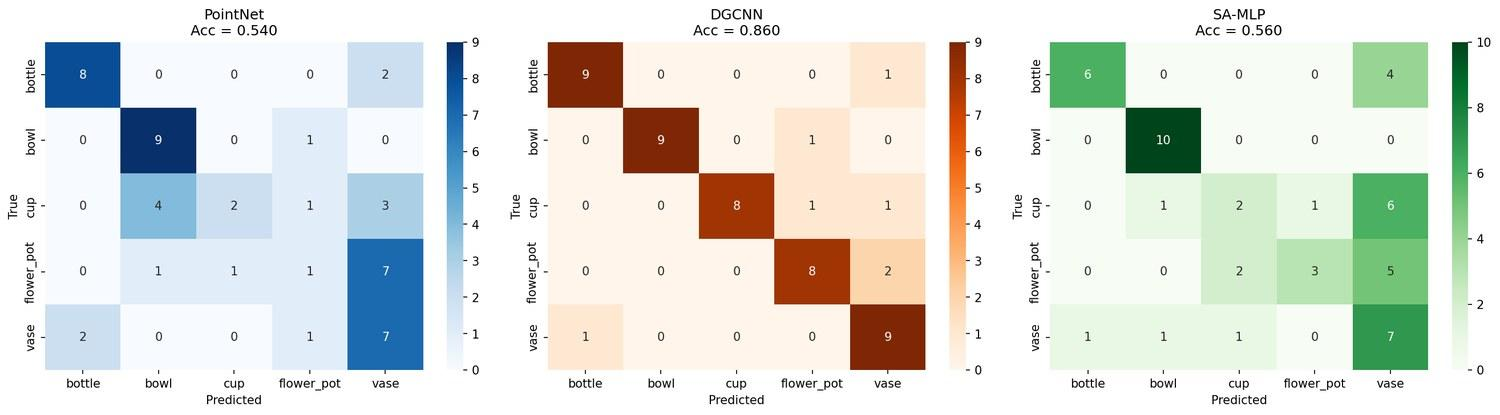
\includegraphics[width=\columnwidth]{figures/fig10.jpg}
  \caption{Матрицы ошибок на реальных сканах}
  \label{fig:real_cm}
\end{figure}

\section{Анализ результатов}

На чистых синтетических данных все три архитектуры показывают близкие результаты: разброс OA составляет 2.3 п.п. Поэтому по одной только точности на чистом синтетическом наборе нельзя обоснованно выбрать архитектуру для практического применения. SA-MLP достигает конкурентного качества при наименьшем числе параметров.

Эксперимент с шумом выявляет компромисс «точность -- устойчивость». PointNet, показывающий наихудший baseline, наиболее устойчив к равномерному аддитивному шуму. Одним из возможных объяснений является глобальный max-pooling: PointNet не моделирует явные локальные отношения между соседними точками, поэтому отдельные локальные геометрические искажения могут оказывать меньшее влияние на итоговое представление. DGCNN и SA-MLP, более точные на чистых данных, резко деградируют при $\sigma\geq0.05$, что может быть связано с нарушением локальных окрестностей, используемых при построении графа соседства и ball query.

Перенос на реальные сканы даёт результат, противоположный шумовому эксперименту. Вероятной причиной является то, что реальный доменный сдвиг — это не аддитивный случайный шум, а качественно иное изменение распределения геометрии: реальные реконструкции могут характеризоваться неравномерной плотностью точек, тогда как ModelNet40 содержит сэмплированные поверхности. Одним из возможных объяснений хорошего переноса DGCNN может быть использование $k$ ближайших соседей: локальные отношения между точками формируются относительно их положения в окрестности, что потенциально снижает зависимость представления от абсолютной плотности сэмплирования. Однако данная гипотеза требует отдельной проверки. Снижение качества при переносе с синтетических на реальные данные также наблюдается в других задачах компьютерного зрения [13,17]. Аналогичная задача распознавания объектов в реальном времени на основе глубоких нейронных сетей решалась и в работах преподавателей кафедры АСУ [21].

Из наблюдений следует практический вывод: в рамках рассматриваемой задачи результаты на синтетическом бенчмарке не позволили надёжно предсказать поведение моделей на реальных сканах. Для задач цифровизации культурного наследия оценка на реальном домене является важной частью сравнительного анализа.

\section{Ограничения исследования}

Размер собственного набора реальных сканов (50 объектов, по 10 на класс) невелик и не позволяет сделать строгих статистических выводов о величинах падения точности. Обучающая выборка ограничена пятью классами из 40 и несбалансирована. Предложенные механистические объяснения (неравномерная плотность как причина сдвига, глобальный max-pooling как источник шумоустойчивости) являются гипотезами, согласующимися с наблюдениями, а не доказанными утверждениями. Наконец, эксперименты проведены в едином прогоне без усреднения по нескольким случайным инициализациям обучения, что ограничивает оценку дисперсии результатов базового бенчмарка.

\section{Заключение}

В работе проведено сравнительное исследование трёх нейросетевых архитектур — PointNet, DGCNN и SA-MLP — в задаче классификации 3D-моделей сосудов-артефактов по облакам точек. Модели обучены по одному экспериментальному протоколу на подмножестве ModelNet40 и оценены в трёх режимах: на чистых данных, при контролируемом гауссовом шуме (mean $\pm$ std по 10 seed'ам) и на независимом наборе из 50 реальных 3D-сканов.

На чистых данных все три модели показали близкую точность (84.6--86.9\%). Эксперименты с шумом и реальными данными выявили различия: PointNet наиболее устойчив к синтетическому шуму (−2.8 п.п. при $\sigma=0.05$), но теряет 30.6 п.п. на реальных сканах. DGCNN, уязвимый к синтетическому шуму (−21.1 п.п. при $\sigma=0.05$), единственный сохраняет точность на реальных данных (−0.9 п.п.). В рассматриваемом эксперименте высокая устойчивость к синтетическому координатному шуму не являлась надёжным индикатором устойчивости к реальному доменному сдвигу. Таким образом, для практической задачи классификации реальных 3D-сканов объектов культурного наследия наиболее предпочтительной архитектурой из трёх рассмотренных является DGCNN, поскольку именно устойчивость к реальному доменному сдвигу, а не к синтетическому зашумлению, определяет применимость модели в условиях эксплуатации.

Направления дальнейшей работы: расширение набора реальных сканов; исследование стратегий сэмплинга для стабильного захвата мелких деталей; методы доменной адаптации; включение трансформерных архитектур в сравнение.

\begin{thebibliography}{99}
\bibitem{ref1} H. Su, S. Maji, E. Kalogerakis, E. Learned-Miller, ``Multi-view Convolutional Neural Networks for 3D Shape Recognition,'' ICCV, 2015, pp. 945--953.
\bibitem{ref2} C. R. Qi, H. Su, K. Mo, L. J. Guibas, ``PointNet: Deep Learning on Point Sets for 3D Classification and Segmentation,'' CVPR, 2017, pp. 652--660.
\bibitem{ref3} C. R. Qi, L. Yi, H. Su, L. J. Guibas, ``PointNet++: Deep Hierarchical Feature Learning on Point Sets in a Metric Space,'' NeurIPS, 2017, pp. 5099--5108.
\bibitem{ref4} Y. Wang, Y. Sun, Z. Liu, S. E. Sarma, M. M. Bronstein, J. M. Solomon, ``Dynamic Graph CNN for Learning on Point Clouds,'' ACM Transactions on Graphics, vol. 38, no. 5, pp. 1--12, 2019.
\bibitem{ref5} H. Zhao, L. Jiang, J. Jia, P. Torr, V. Koltun, ``Point Transformer,'' ICCV, 2021, pp. 16259--16268.
\bibitem{ref6} Z. Wu, S. Song, A. Khosla, F. Yu, L. Zhang, X. Tang, J. Xiao, ``3D ShapeNets: A Deep Representation for Volumetric Shapes,'' CVPR, 2015, pp. 1912--1920.
\bibitem{ref7} A. X. Chang, T. Funkhouser, L. Guibas et al., ``ShapeNet: An Information-Rich 3D Model Repository,'' arXiv:1512.03012, 2015.
\bibitem{ref8} R. Pierdicca, M. Paolanti, F. Matrone et al., ``Point Cloud Semantic Segmentation Using a Deep Learning Framework for Cultural Heritage,'' Remote Sensing, vol. 12, no. 6, p. 1005, 2020.
\bibitem{ref9} D. Maturana, S. Scherer, ``VoxNet: A 3D Convolutional Neural Network for Real-Time Object Recognition,'' IROS, 2015, pp. 922--928.
\bibitem{ref10} Y. Li, R. Bu, M. Sun, W. Wu, X. Di, B. Chen, ``PointCNN: Convolution On X-Transformed Points,'' NeurIPS, 2018, pp. 820--830.
\bibitem{ref11} W. Wu, Z. Qi, L. Fuxin, ``PointConv: Deep Convolutional Networks on 3D Point Clouds,'' CVPR, 2019, pp. 9621--9630.
\bibitem{ref12} M. Guo, J. Cai, Z. Liu, T. Mu, R. R. Martin, S. Hu, ``PCT: Point Cloud Transformer,'' Computational Visual Media, vol. 7, no. 2, pp. 187--199, 2021.
\bibitem{ref13} A. Torralba, A. A. Efros, ``Unbiased Look at Dataset Bias,'' CVPR, 2011, pp. 1521--1528.
\bibitem{ref14} X. Ma, C. Qin, H. You, H. Ran, Y. Fu, ``Rethinking Network Design and Local Geometry in Point Cloud: A Simple Residual MLP Framework,'' ICLR, 2022.
\bibitem{ref15} M. Savva, F. Yu, H. Su et al., ``SHREC'17 Track: Large-Scale 3D Shape Retrieval from ShapeNet Core55,'' Eurographics Workshop on 3D Object Retrieval, 2017.
\bibitem{ref16} К. А. Епифанов, ``Исследование алгоритмов замыкания цикла в лидарной одометрии,'' Искусственный интеллект в промышленных, коммерческих, медицинских и финансовых приложениях: сборник статей научно-технического семинара студентов кафедры «Инженерной кибернетики», вып. 3, НИТУ «МИСиС», 2024, с. 57--61.
\bibitem{ref17} С. Аскари Хеммат, ``Применение синтетических данных из UnrealEngine для обучения модели сегментации мебели,'' Искусственный интеллект в промышленных, коммерческих, медицинских и финансовых приложениях: сборник статей научно-технического семинара студентов кафедры «Инженерной кибернетики», вып. 4, НИТУ «МИСиС», 2025, с. 13--16.
\bibitem{ref18} Р. Р. Бикмаев, М. Д. Золотов, А. Н. Попов, Р. Н. Садеков, ``Повышение точности сопровождения подвижных объектов с применением алгоритма комплексной обработки сигналов с монокулярной камеры и лидара,'' XXVI Санкт-Петербургская международная конференция по интегрированным навигационным системам, 2019, с. 39--42.
\bibitem{ref19} L. E. Alekseev, ``Recognition of scooters in real time using YOLO: a comparative analysis of YOLOv10, YOLOv11,'' Artificial Intelligence in Industrial, Commercial, Medical and Financial Applications, NUST MISIS, 2025, pp. 4--7.
\bibitem{ref20} I. M. Bakhvalov, S. V. Startsev, ``Recognition of UAVs of various classes by means of computer vision,'' Artificial Intelligence in Industrial, Commercial, Medical and Financial Applications, NUST MISIS, 2024, pp. 34--40.
\bibitem{ref21} I. O. Temkin, M. O. Antonov, ``Recognition and tracking of road surface defects in real time based on the integrated use of standard computational procedures and deep neural networks,'' Programmnye produkty i sistemy, no. 3, pp. 421--430, 2024.
\bibitem{ref22} S. M. Khlobustova, ``sketchfab\_model: real-world 3D scans of vessel artifacts (bottle, bowl, cup, flower\_pot, vase),'' Kaggle, 2026. [Online]. Available: \url{https://www.kaggle.com/datasets/khlobustovasvetlana/sketchfab-model}.
\end{thebibliography}

\end{document}
